\documentclass[11pt]{article}

\usepackage[margin=1in]{geometry}
\usepackage[T1]{fontenc}
\usepackage{mathpazo}
\usepackage{microtype}
\usepackage{amsmath}
\usepackage{amssymb}
\usepackage{booktabs}
\usepackage{array}
\usepackage{siunitx}
\sisetup{table-number-alignment=center, table-format=2.2}
\usepackage{enumitem}
\usepackage{float}
\usepackage{graphicx}
\usepackage{hyperref}
\usepackage{xcolor}
\usepackage{caption}
\usepackage{tikz}
\usetikzlibrary{arrows.meta, shapes.geometric, positioning, fit, backgrounds}
\usepackage{fancyhdr}
\usepackage{titlesec}

\linespread{1.05}
\setlength{\parindent}{1.5em}
\setlength{\parskip}{4pt}

% Section heading style
\titleformat{\section}{\large\bfseries}{\thesection}{1em}{}
\titlespacing*{\section}{0pt}{20pt}{8pt}
\titleformat{\subsection}{\normalsize\bfseries}{\thesubsection}{1em}{}
\titlespacing*{\subsection}{0pt}{12pt}{4pt}

\hypersetup{
  colorlinks=true,
  linkcolor=blue!50!black,
  citecolor=blue!50!black,
  urlcolor=blue!50!black
}

\captionsetup{
  font=small,
  labelfont=bf
}

\title{\textbf{A Modular Quantitative Trading Pipeline:}\\
\Large Alpha Generation, Reinforcement Learning Control, and Risk-Aware Backtesting}
\author{
Ioan Hedea\\
\small Sequential Decision-Making Project
}
\date{March 2026}

\pagestyle{fancy}
\fancyhf{}
\fancyhead[L]{\small\itshape Ioan Hedea}
\fancyhead[R]{\small\itshape A Modular Quantitative Trading Pipeline}
\fancyfoot[C]{\small\thepage}
\renewcommand{\headrulewidth}{0.4pt}

\begin{document}
\maketitle
\thispagestyle{plain}

\begin{abstract}
This paper documents a modular quantitative trading pipeline implemented in
\texttt{quant\_stack}, a module within the \texttt{stock\_trading} package. The system combines
cross-sectional factor investing, cointegration-based statistical arbitrage,
volatility forecasting, regime detection, and a lightweight recurrent forecast
sleeve with reinforcement-learning-based portfolio allocation, hedging, and
execution components. The design is intentionally hybrid: classical quantitative
finance supplies the alpha and risk features, while reinforcement learning is
used as a sequential control layer for exposure, overlay intensity, and
tail-risk management. On the current backtest window, the full pipeline attains
equity-like return with a materially improved drawdown profile relative to SPY,
while remaining close to the strongest factor-only benchmark in upside capture.
\end{abstract}

\medskip
\noindent\textbf{Keywords:} quantitative trading, reinforcement learning, factor investing, statistical arbitrage, regime detection, risk management, backtesting

\bigskip\noindent\rule{\textwidth}{0.4pt}\bigskip

\section{Introduction}

Many quantitative trading systems are built from a collection of specialized
modules rather than from a single monolithic predictor. Cross-sectional factors,
relative-value signals, volatility models, and regime filters often contribute
distinct pieces of information about expected return and risk. Reinforcement
learning (RL), by contrast, is most compelling when the task is inherently
sequential: choosing when to increase risk, when to hedge, and how to adapt
execution to changing conditions \cite{sutton2018,almgren2000}.

This project adopts exactly that separation of responsibilities. The alpha layer
is intentionally finance-first. It draws on ideas from factor investing
\cite{fama1993,jegadeesh1993}, cointegration-based statistical arbitrage
\cite{engle1987}, conditional volatility modeling \cite{engle1982,bollerslev1986},
and regime detection \cite{hamilton1989}. The RL layer does not attempt to
discover alpha from scratch. Instead, it treats alpha as an input and learns how
aggressively to express it under different risk and market states.

The main contributions of the implementation are fourfold.
\begin{enumerate}[leftmargin=1.5em, itemsep=2pt, topsep=4pt]
\item A modular code architecture that cleanly separates data, alpha, control,
      backtesting, and visualization concerns.
\item A factor-anchored portfolio construction policy in which RL primarily
      controls exposure and active overlay size rather than acting as a second
      stock selector.
\item A light dynamic hedging sleeve that delivers convex-protection-like
      behavior without requiring a full options-chain pipeline.
\item A research-style reporting workflow that connects theory, architecture, and
      empirical diagnostics in a reproducible form.
\end{enumerate}

From a research perspective, this framing matters because it narrows the gap
between a teaching prototype and a system that can be discussed in the language
of quantitative portfolio construction. The objective is not to claim that the
pipeline is production-ready. Rather, it is to assemble a well-motivated stack
in which each modeling choice has a clear financial role and where performance
can be decomposed into alpha generation, risk transformation, and control.

\section{Related Literature and Design Motivation}

The report is not meant to claim novelty in any individual modeling choice.
Instead, it builds a coherent pipeline from well-established ingredients.

\textbf{Factor investing.} The cross-sectional component is aligned with the idea
that common risk factors help explain returns \cite{fama1993}. Momentum is
motivated by the medium-horizon continuation evidence of Jegadeesh and Titman
\cite{jegadeesh1993}, while quality and low-volatility proxies are included to
stabilize the cross-section.

\textbf{Statistical arbitrage.} The pairs sleeve follows the classical
cointegration logic of Engle and Granger \cite{engle1987}: if a spread is mean
reverting around an equilibrium relation, deviations from that equilibrium may
carry predictive content.

\textbf{Volatility and regimes.} Conditional heteroskedasticity motivates the
GARCH sleeve \cite{engle1982,bollerslev1986}, while the market-regime component
uses a two-state hidden Markov model in the spirit of Hamilton \cite{hamilton1989}.

\textbf{Reinforcement learning.} RL is used as a controller rather than a raw
alpha generator. This follows the practical observation that in finance, RL is
often most useful for allocation, inventory, and execution decisions rather than
for replacing domain-specific signal construction \cite{sutton2018,almgren2000}.

\section{System Architecture}

The pipeline is organized as a linear sequence of stages, illustrated in
Figure~\ref{fig:architecture}. Each stage has a clearly delimited responsibility:
upstream stages produce signals and risk features, the control layer translates
these into portfolio decisions, and the backtest layer evaluates realized
outcomes.

\begin{figure}[H]
\centering
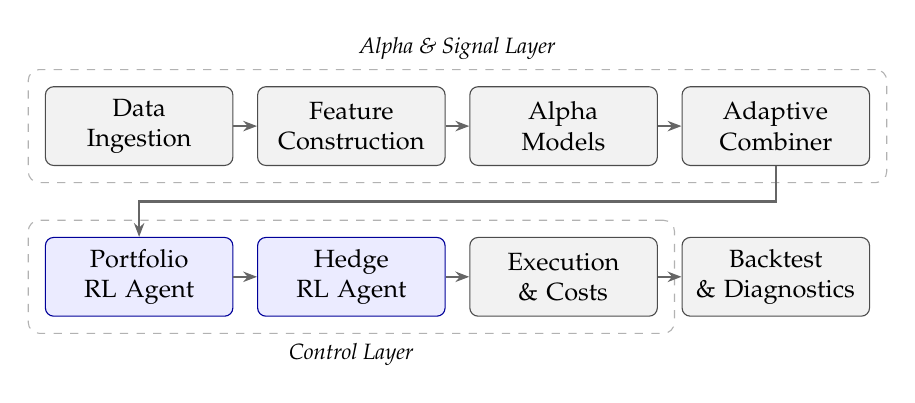
\begin{tikzpicture}[
  node distance = 0.45cm and 0.30cm,
  box/.style = {
    rectangle, rounded corners=3pt,
    draw=black!70, fill=gray!10,
    text width=2.1cm, align=center,
    font=\small, minimum height=1.0cm,
    inner sep=4pt
  },
  rlbox/.style = {
    rectangle, rounded corners=3pt,
    draw=blue!60!black, fill=blue!8,
    text width=2.1cm, align=center,
    font=\small, minimum height=1.0cm,
    inner sep=4pt
  },
  arr/.style = {-{Stealth[length=5pt]}, thick, black!60},
  groupbox/.style = {
    draw=black!30, dashed, rounded corners=4pt,
    fill=none, inner sep=6pt
  }
]

% Row 1: Data → Features → Alpha Models → Adaptive Combiner
\node[box] (data)    {Data\\Ingestion};
\node[box, right=of data]    (feat)    {Feature\\Construction};
\node[box, right=of feat]    (alpha)   {Alpha\\Models};
\node[box, right=of alpha]   (comb)    {Adaptive\\Combiner};

% Row 2: Portfolio RL → Hedge/Cash → Backtest
\node[rlbox, below=0.9cm of data]  (portrl)  {Portfolio\\RL Agent};
\node[rlbox, right=of portrl]      (hedgerl) {Hedge\\RL Agent};
\node[box,   right=of hedgerl]     (exec)    {Execution\\\& Costs};
\node[box,   right=of exec]        (bt)      {Backtest\\\& Diagnostics};

% Row 1 arrows
\draw[arr] (data)  -- (feat);
\draw[arr] (feat)  -- (alpha);
\draw[arr] (alpha) -- (comb);

% Combiner down to portfolio RL
\draw[arr] (comb.south) -- ++(0,-0.45) -| (portrl.north);

% Row 2 arrows
\draw[arr] (portrl)  -- (hedgerl);
\draw[arr] (hedgerl) -- (exec);
\draw[arr] (exec)    -- (bt);

% Labels
\begin{scope}[on background layer]
  \node[groupbox, fit=(data)(feat)(alpha)(comb),
        label={[font=\footnotesize\itshape]above:Alpha \& Signal Layer}] {};
  \node[groupbox, fit=(portrl)(hedgerl)(exec),
        label={[font=\footnotesize\itshape]below:Control Layer}] {};
\end{scope}
\end{tikzpicture}
\caption{High-level architecture of the quantitative trading pipeline. The alpha
and signal layer (top) produces expected-return scores and risk features; the
control layer (bottom) translates these into portfolio weights, hedge intensity,
and cash allocation before evaluation in the backtest engine.}
\label{fig:architecture}
\end{figure}

\subsection{Software Structure}

\begin{table}[H]
\centering
\caption{Module-level decomposition of the \texttt{quant\_stack} package.}
\begin{tabular}{@{} l p{9.5cm} @{}}
\toprule
\textbf{Module} & \textbf{Responsibility} \\
\midrule
\texttt{config.py}   & Universe definition, global constants, and external series identifiers \\
\texttt{data.py}     & Market price/volume ingestion, macro series (FRED / BLS fallback), and SEC company facts \\
\texttt{alpha.py}    & Cross-sectional factors, pairs cointegration, GARCH volatility, HMM regime, LSTM forecast, and adaptive signal combination \\
\texttt{rl.py}       & Portfolio construction agent, execution controller, and dynamic hedging agent \\
\texttt{pipeline.py} & Walk-forward backtest orchestration and online RL update loop \\
\texttt{plots.py}    & Equity-curve, drawdown, RL behavior, and alpha-model diagnostic figures \\
\texttt{main.py}     & CLI entry point and compatibility wrapper \\
\bottomrule
\end{tabular}
\end{table}

This decomposition is important for research reproducibility. It keeps the
external command stable while turning the internals into separately testable
components.

\section{Data and Feature Construction}

\subsection{Universe}

The traded universe spans four broad buckets. The growth sleeve comprises AAPL,
MSFT, GOOGL, AMZN, META, and NVDA. Financials and energy are represented by JPM,
GS, XOM, and CVX. The defensive sleeve includes JNJ, PG, KO, PEP, and WMT, while
diversifiers are captured through GLD, TLT, XLU, and VNQ. SPY serves as the
passive equity benchmark throughout.

\subsection{Data Sources}

The pipeline supports both a free baseline configuration and a richer research
configuration. Daily prices and volumes are sourced via \texttt{yfinance}. When a
\texttt{FRED\_API\_KEY} is available, macro data are drawn directly from FRED; in
its absence, the system falls back to BLS and U.S.\ Treasury Fiscal Data. SEC
company facts are incorporated when \texttt{SEC\_USER\_AGENT} is set, enabling a
light fundamentals layer without requiring a proprietary data subscription.

\subsection{Macro Regime Inputs}

When available, the macro sleeve includes rates and labor-market variables such
as the 10-year yield, 2-year yield, federal funds rate, unemployment rate, and
term spread. These variables do not form a standalone alpha book. Instead, they
help create a macro regime belief that is blended with the HMM regime estimate.

\section{Methodology}

\subsection{Problem Formulation}

Let $r_{t+1} \in \mathbb{R}^N$ denote next-period asset returns for a universe of
$N$ tradable assets. At time $t$, the system observes a feature state
$x_t \in \mathcal{X}$ constructed from cross-sectional factor values,
relative-value spreads, volatility forecasts, regime beliefs, and macro inputs.
The alpha layer maps these features into an expected-return score vector
$\alpha_t \in \mathbb{R}^N$ and a confidence vector $c_t \in \mathbb{R}^N$.

The control layer then chooses a portfolio allocation $w_t$, a cash allocation,
and a hedge intensity $h_t$. The one-step portfolio objective is not written as
a pure return maximization problem. Instead, it is implicitly multi-objective:
maximize long-run wealth while limiting drawdown, volatility, and unnecessary
turnover. This is the reason the project separates alpha estimation from control:
the two tasks operate on different time scales and carry different inductive
biases.

\subsection{Cross-Sectional Factor Model}

The factor sleeve combines four z-scored components: momentum, a value proxy, a
quality proxy, and a low-volatility tilt. Letting $m_i$, $v_i$, $q_i$, and
$\ell_i$ denote the standardized scores for asset
$i$, the composite factor score is
\[
f_i = 0.30 m_i + 0.25 v_i + 0.25 q_i + 0.20 \ell_i.
\]

This choice reflects a balanced, multi-style factor book rather than a single
directional bet.

\subsection{Pairs Trading}

For candidate pairs, a hedge ratio $\beta$ is estimated by OLS and the spread
\[
s_t = P^{(1)}_t - \beta P^{(2)}_t
\]
is normalized into a z-score
\[
z_t = \frac{s_t - \mu_s}{\sigma_s + \varepsilon}.
\]
Large positive z-scores correspond to short-spread trades and large negative
z-scores correspond to long-spread trades.

\subsection{Volatility and Regime Models}

Each name receives a GARCH(1,1) forecast
\[
\sigma_t^2 = \omega + \alpha_1 \epsilon_{t-1}^2 + \beta_1 \sigma_{t-1}^2,
\]
where $\omega > 0$, $\alpha_1 \geq 0$, and $\beta_1 \geq 0$ are the intercept,
ARCH, and GARCH coefficients respectively. This conditional variance estimate
is used for confidence scaling and risk awareness. Separately, a two-state
HMM produces a bull-versus-bear regime belief. The final regime signal is
\[
\text{RegimeBelief}_t =
0.75 \cdot \text{HMMBelief}_t +
0.25 \cdot \text{MacroBelief}_t.
\]

\subsection{Adaptive Alpha Combination}

Let $s^{(k)}_{i,t}$ denote the signal from source $k$ for asset $i$ at time $t$.
The expected return score is formed as
\[
\alpha_{i,t} = \sum_k w^{(k)}_t s^{(k)}_{i,t},
\]
where the source weights $w^{(k)}_t$ adapt over time based on recent realized
signal quality. In the implementation, this is proxied by recent Spearman
information coefficients between source scores and realized returns.

This adaptive weighting is important because the constituent alpha sleeves are
not equally informative across all market states. Pairs signals can be weak in
strongly trending markets, deep nonlinear forecasts can degrade when regime
structure shifts, and factor signals can vary in efficacy depending on the
dispersion of the cross-section. The adaptive combiner therefore behaves like a
simple online model-selection layer.

\subsection{Portfolio Construction RL}

The portfolio RL state summarizes three inputs: the current cross-sectional alpha
opportunity, recent realized portfolio volatility, and the prevailing regime
belief. Crucially, the policy is \emph{factor-anchored}. The target book is
\[
w_t^{\text{target}} =
0.90\,w_t^{\text{factor}} +
0.10\,w_t^{\text{stabilizer}},
\]
where the stabilizer is a long-only minimum-variance-style portfolio estimated
from a Ledoit--Wolf shrinkage covariance matrix.

If the RL agent chooses invested fraction $b_t$ and active overlay size $\tau_t$,
the final invested portfolio is approximately
\[
w_t =
b_t \left[(1-\tau_t)w_t^{\text{target}} + \tau_t w_t^{\text{satellite}}\right].
\]
The satellite sleeve is not a fully independent book; it tilts the factor target
toward the strongest alpha names. This keeps the full pipeline close to the
working factor engine while still letting RL modulate aggressiveness.

\subsection{Reward Design}

The portfolio RL update uses a differential Sharpe-style reward based on the
realized portfolio return relative to a recent rolling distribution of returns.
This means the agent is not rewarded solely for taking more risk in absolute
terms; it is rewarded for improving return relative to the recent volatility
environment. The hedge agent uses an asymmetric realized-return reward in which
losses are penalized more heavily than gains are rewarded. That asymmetry is a
deliberate design choice: it pushes the hedge layer toward preserving capital in
stress rather than maximizing average carry.

\subsection{No-Trade Band and Hedging}

To reduce turnover drag, a rebalance band suppresses small changes in target
weights. When only part of the portfolio is changed, the active weights are
rescaled to preserve the desired capital budget.

The hedging RL layer observes drawdown, volatility regime, and recent momentum.
It chooses one of four hedge intensities. The total one-period return can be
written schematically as
\[
r_t^{\text{total}} =
r_t^{\text{risky}}(1-\phi h_t) + r_t^{\text{cash}} + r_t^{\text{hedge}},
\]
where $h_t$ is the hedge fraction and $r_t^{\text{hedge}}$ includes both carry
cost and a convex stress payoff approximation.

Although stylized, this formulation captures the intended economics of a
protection sleeve: hedging should be mildly costly in calm periods, increasingly
helpful in volatile or negative markets, and most valuable when drawdowns and
adverse momentum coincide.

\section{Experimental Design}

The backtest uses a walk-forward protocol over approximately five years of daily
data. The sample is split evenly into training and test segments. The LSTM
sleeve is first trained on the initial window, after which the full pipeline is
rolled forward one trading day at a time.

At each date, the pipeline executes the following sequence. First, factor, pairs,
GARCH, HMM, macro, and LSTM features are generated from the available data.
These are combined into expected-return scores and confidence levels via the
adaptive combiner. The portfolio RL agent then selects an exposure bucket and
overlay size, after which the hedging agent independently chooses the hedge
intensity. Transaction costs, cash carry, and hedge payoffs are applied to arrive
at the realized portfolio return, which is finally used to update both RL value
tables before advancing to the next trading day.

The comparison set includes SPY buy-and-hold, an equal-weight benchmark, and a
factor-only strategy with no RL overlay.

\subsection{Benchmark Logic}

The benchmark set is chosen to isolate different sources of value. SPY measures
whether the pipeline adds value relative to a standard passive equity exposure.
Equal weight tests whether the broadened universe alone produces useful
diversification benefits. Factor-only isolates the pure alpha layer without any
RL overlay. Comparing the full pipeline against factor-only is particularly
important because it reveals whether RL is adding value as a controller or merely
acting as a drag on a strong stock-selection engine.

\subsection{Transaction Costs and Carry}

The backtest includes a simple turnover-based transaction-cost model and daily
risk-free carry on uninvested cash. These assumptions remain stylized, but they
are sufficient to force the allocator to confront a meaningful trade-off between
responsiveness and trading friction. The no-trade band is best understood in this
context: it is not just an implementation convenience, but a structural attempt
to reduce noise trading in a daily-rebalanced system.

\section{Evaluation Metrics}

The reporting suite includes annualized return, annualized volatility, Sharpe
ratio, Sortino ratio, maximum drawdown, Calmar ratio, and return-distribution
diagnostics including a daily 5\% Value-at-Risk estimate.

If $\{r_t\}_{t=1}^T$ denotes daily portfolio returns and $r_f$ is the annual
risk-free rate, then the annualized Sharpe ratio is
\[
\text{Sharpe} = \frac{252 \, \bar{r} - r_f}{\sqrt{252}\,\hat{\sigma}(r) + \varepsilon}.
\]
The Sortino ratio replaces total volatility with downside volatility, while the
Calmar ratio scales annualized return by the magnitude of maximum drawdown. Each
metric emphasizes a different aspect of the return distribution, which matters in
this project because the pipeline is explicitly designed to reshape tail risk,
not merely to maximize mean return.

\section{Results}

The most recent strong run uses a test window from September 20, 2023 to
March 23, 2026. The summary metrics are shown in Table~\ref{tab:metrics}.

\begin{table}[H]
\centering
\caption{Performance summary on the walk-forward test window
  (20 Sep 2023 -- 23 Mar 2026). Annualized figures. Max DD denotes maximum
  peak-to-trough drawdown; Calmar is annualized return divided by $|\text{Max DD}|$.}
\label{tab:metrics}
\begin{tabular}{@{} l r r r r r @{}}
\toprule
\textbf{Strategy} & \textbf{Return} & \textbf{Volatility} & \textbf{Sharpe} & \textbf{Max DD} & \textbf{Calmar} \\
\midrule
Full Pipeline & 32.0\% & 12.9\% & 2.21 & $-$11.7\% & 2.72 \\
Factor Only   & 33.4\% & 15.3\% & 1.96 & $-$16.5\% & 2.03 \\
Equal Weight  & 22.7\% & 11.7\% & 1.63 & $-$14.8\% & 1.53 \\
SPY           & 18.4\% & 15.7\% & 0.95 & $-$18.8\% & 0.98 \\
\bottomrule
\end{tabular}
\end{table}

The key interpretation is that the full pipeline retains most of the upside of
the factor-only strategy while materially reducing drawdown and volatility.
Relative to SPY, the pipeline improves both return and risk-adjusted
performance. Relative to the factor-only benchmark, it gives up a small amount
of raw return in exchange for better risk control.

The resulting profile is informative. The factor-only strategy remains the most
aggressive expression of the alpha book, which is consistent with its higher
volatility and deeper drawdown. The full pipeline, by contrast, sits closer to
what one would expect from an institutional overlay: it captures much of the
equity upside, preserves a strong Sharpe ratio, and converts some of the raw
return advantage into a shallower left tail.

Figures~\ref{fig:rl}--\ref{fig:execution} provide further behavioral detail.
The RL diagnostics (Figure~\ref{fig:rl}) confirm that both the portfolio and
hedge agents vary their actions in a regime-consistent manner rather than
converging to a fixed policy. The alpha model diagnostics (Figure~\ref{fig:alpha})
illustrate how the adaptive combiner shifts weight toward sleeves with higher
recent information coefficients. The execution RL panel
(Figure~\ref{fig:execution}) shows that the no-trade band meaningfully reduces
turnover relative to unconstrained daily rebalancing, with the cost savings
concentrated in low-alpha-conviction periods.

\begin{figure}[H]
\centering

\includegraphics[width=\textwidth]{stock_trading/pipeline_performance.png}
\caption{Performance comparison for the full pipeline and benchmark strategies.}
\label{fig:performance}
\end{figure}

\begin{figure}[H]
\centering

\includegraphics[width=\textwidth]{stock_trading/pipeline_rl_analysis.png}
\caption{Behavioral diagnostics for the portfolio and hedging RL layers.}
\label{fig:rl}
\end{figure}

\begin{figure}[H]
\centering

\includegraphics[width=\textwidth]{stock_trading/pipeline_alpha_models.png}
\caption{Alpha model diagnostics: per-sleeve signal quality and adaptive combination weights over the test window.}
\label{fig:alpha}
\end{figure}

\begin{figure}[H]
\centering

\includegraphics[width=\textwidth]{stock_trading/pipeline_execution_rl.png}
\caption{Execution RL layer: turnover management, no-trade band activations, and realized transaction-cost drag.}
\label{fig:execution}
\end{figure}

\section{Discussion}

The experimental results support two conclusions of particular methodological importance.

First, the data and alpha side of the pipeline is doing real work. The
factor-only benchmark is strong, and equal-weight also performs well, suggesting
that the broader universe and adaptive alpha combination add meaningful signal.

Second, the latest factor-anchored RL design improves the role of the control
layer. Earlier versions were too defensive and suppressed upside. The current
version behaves more like an institutional overlay: it keeps the strategy close
to the factor book, but uses RL to modulate exposure and hedge intensity when the
market state becomes less favorable.

This distinction is central. If the RL layer were treated as a second stock
selector, it would risk duplicating the alpha problem with a less structured
model and less data efficiency. By anchoring the policy to the factor book, the
pipeline preserves interpretability: alpha determines \emph{what} to own, while
RL primarily determines \emph{how much} to own and \emph{how much protection} to
carry.

The results also suggest a useful practical lesson. Improvements in data quality
and signal specification are likely to matter more from this point onward than
adding more control complexity. The current architecture is already rich enough
to express nontrivial risk management behavior. Future gains will likely come
from more realistic point-in-time fundamentals, macro release lags, cross-asset
regime features, and richer hedging instruments.

\section{Limitations and Future Work}

The implementation remains research code, and several caveats apply. Macro inputs
are not yet fully vintage-aware or release-lagged, and SEC enrichment does not
yet constitute a true point-in-time fundamentals database. Transaction costs
remain stylized rather than venue-specific. The hedge sleeve approximates convex
protection without live options data, and the evaluation still reflects a single
realized market path rather than a distribution of out-of-sample windows.

Natural next steps include point-in-time fundamentals, release-lagged macro
features, cross-asset regime instruments, and a more realistic hedge sleeve
using options or implied-volatility information.

An additional research direction would be to evaluate robustness across rolling
subperiods instead of relying on a single aggregate test window. That would make
it easier to distinguish structural improvements from favorable alignment with a
particular market regime.

\section{Conclusion}

This project demonstrates that a financially grounded hybrid architecture can be
both modular and effective. Classical quantitative models remain responsible for
alpha discovery, while reinforcement learning acts as a sequential risk and
allocation controller. The resulting system is not simply a benchmark chaser; it
is a structured research pipeline whose behavior is interpretable, testable, and
extensible.

\appendix

\section{Implementation Snapshot}

\subsection{Current RL Control Ladders}

\begin{center}
\begin{tabular}{lcc}
\toprule
Portfolio action & Invested fraction & Active overlay fraction \\
\midrule
State 0 & 82\% & 5\% \\
State 1 & 90\% & 8\% \\
State 2 & 95\% & 12\% \\
State 3 & 98\% & 16\% \\
State 4 & 100\% & 20\% \\
\bottomrule
\end{tabular}
\end{center}

\begin{center}
\begin{tabular}{lc}
\toprule
Hedge action & Hedge ratio \\
\midrule
State 0 & 0\% \\
State 1 & 3\% \\
State 2 & 8\% \\
State 3 & 15\% \\
\bottomrule
\end{tabular}
\end{center}

\begin{thebibliography}{99}

\bibitem{almgren2000}
R. Almgren and N. Chriss.
\newblock Optimal execution of portfolio transactions.
\newblock \emph{Journal of Risk}, 3(2):5--39, 2000.

\bibitem{bollerslev1986}
T. Bollerslev.
\newblock Generalized autoregressive conditional heteroskedasticity.
\newblock \emph{Journal of Econometrics}, 31(3):307--327, 1986.

\bibitem{engle1982}
R. F. Engle.
\newblock Autoregressive conditional heteroscedasticity with estimates of the
  variance of United Kingdom inflation.
\newblock \emph{Econometrica}, 50(4):987--1007, 1982.

\bibitem{engle1987}
R. F. Engle and C. W. J. Granger.
\newblock Co-integration and error correction: representation, estimation, and
  testing.
\newblock \emph{Econometrica}, 55(2):251--276, 1987.

\bibitem{fama1993}
E. F. Fama and K. R. French.
\newblock Common risk factors in the returns on stocks and bonds.
\newblock \emph{Journal of Financial Economics}, 33(1):3--56, 1993.

\bibitem{hamilton1989}
J. D. Hamilton.
\newblock A new approach to the economic analysis of nonstationary time series
  and the business cycle.
\newblock \emph{Econometrica}, 57(2):357--384, 1989.

\bibitem{jegadeesh1993}
N. Jegadeesh and S. Titman.
\newblock Returns to buying winners and selling losers: implications for stock
  market efficiency.
\newblock \emph{Journal of Finance}, 48(1):65--91, 1993.

\bibitem{sutton2018}
R. S. Sutton and A. G. Barto.
\newblock \emph{Reinforcement Learning: An Introduction}.
\newblock MIT Press, Cambridge, MA, second edition, 2018.

\end{thebibliography}

\end{document}
